% Created by tikzDevice version 0.12.6 on 2026-08-08 13:32:32
% !TEX encoding = UTF-8 Unicode
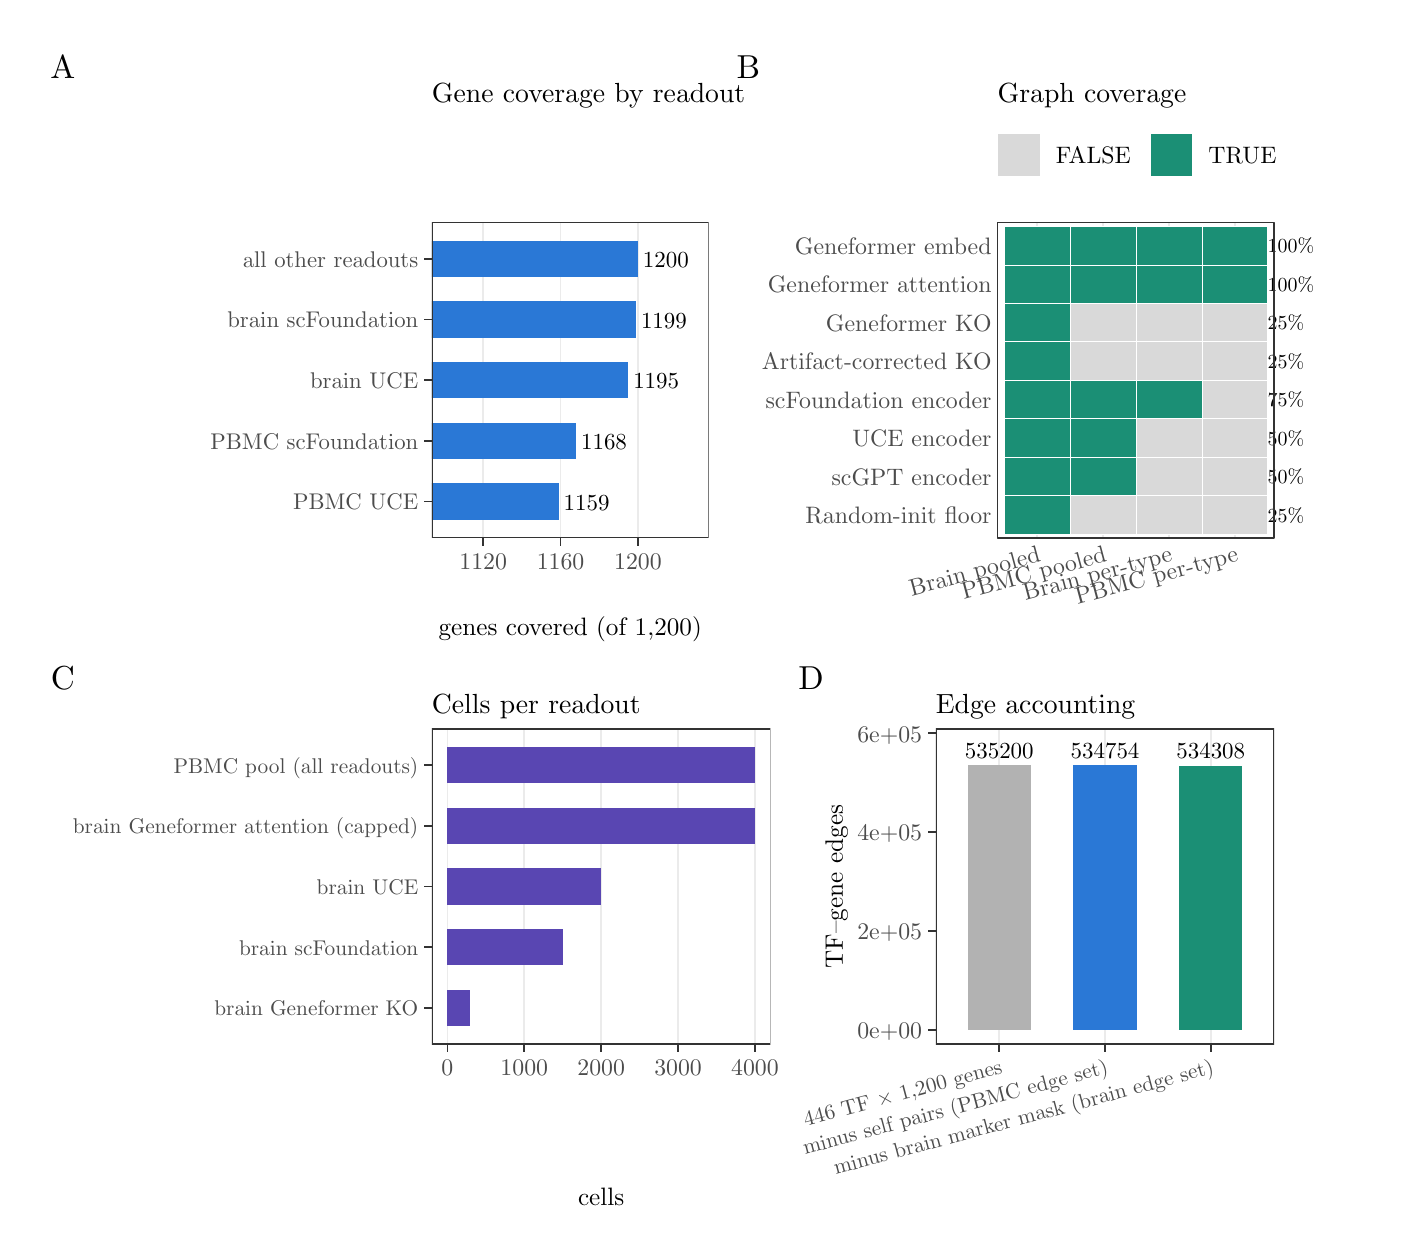
\begin{tikzpicture}[x=1pt,y=1pt]
\definecolor{fillColor}{RGB}{255,255,255}
\path[use as bounding box,fill=fillColor,fill opacity=0.00] (0,0) rectangle (491.44,433.62);
\begin{scope}
\path[clip] (  0.00,  0.00) rectangle (491.44,433.62);
\definecolor{drawColor}{RGB}{255,255,255}
\definecolor{fillColor}{RGB}{255,255,255}

\path[draw=drawColor,line width= 0.6pt,line join=round,line cap=round,fill=fillColor] ( -0.00,  0.00) rectangle (491.44,433.62);
\end{scope}
\begin{scope}
\path[clip] (  4.00,208.77) rectangle (252.02,429.62);
\definecolor{drawColor}{RGB}{255,255,255}
\definecolor{fillColor}{RGB}{255,255,255}

\path[draw=drawColor,line width= 0.6pt,line join=round,line cap=round,fill=fillColor] (  4.00,208.77) rectangle (252.02,429.62);
\end{scope}
\begin{scope}
\path[clip] (252.02,208.77) rectangle (485.44,429.62);
\definecolor{drawColor}{RGB}{255,255,255}
\definecolor{fillColor}{RGB}{255,255,255}

\path[draw=drawColor,line width= 0.6pt,line join=round,line cap=round,fill=fillColor] (252.02,208.77) rectangle (485.44,429.62);
\end{scope}
\begin{scope}
\path[clip] (146.09,249.22) rectangle (246.02,363.22);
\definecolor{fillColor}{RGB}{255,255,255}

\path[fill=fillColor] (146.09,249.22) rectangle (246.02,363.22);
\definecolor{drawColor}{gray}{0.92}

\path[draw=drawColor,line width= 0.6pt,line join=round] (164.61,249.22) --
	(164.61,363.22);

\path[draw=drawColor,line width= 0.6pt,line join=round] (192.56,249.22) --
	(192.56,363.22);

\path[draw=drawColor,line width= 0.6pt,line join=round] (220.51,249.22) --
	(220.51,363.22);
\definecolor{fillColor}{RGB}{42,120,214}

\path[fill=fillColor] (-618.08,299.64) rectangle (217.02,312.80);

\path[fill=fillColor] (-618.08,321.57) rectangle (219.81,334.72);

\path[fill=fillColor] (-618.08,277.72) rectangle (198.15,290.87);

\path[fill=fillColor] (-618.08,255.80) rectangle (191.86,268.95);

\path[fill=fillColor] (-618.08,343.49) rectangle (220.51,356.64);
\definecolor{drawColor}{RGB}{0,0,0}

\node[text=drawColor,anchor=base west,inner sep=0pt, outer sep=0pt, scale=  0.83] at (218.83,303.16) {1195};

\node[text=drawColor,anchor=base west,inner sep=0pt, outer sep=0pt, scale=  0.83] at (221.63,325.08) {1199};

\node[text=drawColor,anchor=base west,inner sep=0pt, outer sep=0pt, scale=  0.83] at (199.96,281.23) {1168};

\node[text=drawColor,anchor=base west,inner sep=0pt, outer sep=0pt, scale=  0.83] at (193.67,259.31) {1159};

\node[text=drawColor,anchor=base west,inner sep=0pt, outer sep=0pt, scale=  0.83] at (222.33,347.00) {1200};
\definecolor{drawColor}{gray}{0.20}

\path[draw=drawColor,line width= 0.6pt,line join=round,line cap=round] (146.09,249.22) rectangle (246.02,363.22);
\end{scope}
\begin{scope}
\path[clip] (  0.00,  0.00) rectangle (491.44,433.62);
\definecolor{drawColor}{gray}{0.30}

\node[text=drawColor,anchor=base east,inner sep=0pt, outer sep=0pt, scale=  0.82] at (141.14,259.34) {PBMC UCE};

\node[text=drawColor,anchor=base east,inner sep=0pt, outer sep=0pt, scale=  0.82] at (141.14,281.27) {PBMC scFoundation};

\node[text=drawColor,anchor=base east,inner sep=0pt, outer sep=0pt, scale=  0.82] at (141.14,303.19) {brain UCE};

\node[text=drawColor,anchor=base east,inner sep=0pt, outer sep=0pt, scale=  0.82] at (141.14,325.11) {brain scFoundation};

\node[text=drawColor,anchor=base east,inner sep=0pt, outer sep=0pt, scale=  0.82] at (141.14,347.04) {all other readouts};
\end{scope}
\begin{scope}
\path[clip] (  0.00,  0.00) rectangle (491.44,433.62);
\definecolor{drawColor}{gray}{0.20}

\path[draw=drawColor,line width= 0.6pt,line join=round] (143.34,262.37) --
	(146.09,262.37);

\path[draw=drawColor,line width= 0.6pt,line join=round] (143.34,284.30) --
	(146.09,284.30);

\path[draw=drawColor,line width= 0.6pt,line join=round] (143.34,306.22) --
	(146.09,306.22);

\path[draw=drawColor,line width= 0.6pt,line join=round] (143.34,328.14) --
	(146.09,328.14);

\path[draw=drawColor,line width= 0.6pt,line join=round] (143.34,350.07) --
	(146.09,350.07);
\end{scope}
\begin{scope}
\path[clip] (  0.00,  0.00) rectangle (491.44,433.62);
\definecolor{drawColor}{gray}{0.20}

\path[draw=drawColor,line width= 0.6pt,line join=round] (164.61,246.47) --
	(164.61,249.22);

\path[draw=drawColor,line width= 0.6pt,line join=round] (192.56,246.47) --
	(192.56,249.22);

\path[draw=drawColor,line width= 0.6pt,line join=round] (220.51,246.47) --
	(220.51,249.22);
\end{scope}
\begin{scope}
\path[clip] (  0.00,  0.00) rectangle (491.44,433.62);
\definecolor{drawColor}{gray}{0.30}

\node[text=drawColor,anchor=base,inner sep=0pt, outer sep=0pt, scale=  0.86] at (164.61,237.88) {1120};

\node[text=drawColor,anchor=base,inner sep=0pt, outer sep=0pt, scale=  0.86] at (192.56,237.88) {1160};

\node[text=drawColor,anchor=base,inner sep=0pt, outer sep=0pt, scale=  0.86] at (220.51,237.88) {1200};
\end{scope}
\begin{scope}
\path[clip] (  0.00,  0.00) rectangle (491.44,433.62);
\definecolor{drawColor}{RGB}{0,0,0}

\node[text=drawColor,anchor=base,inner sep=0pt, outer sep=0pt, scale=  0.91] at (196.05,213.93) {genes covered (of 1,200)};
\end{scope}
\begin{scope}
\path[clip] (  0.00,  0.00) rectangle (491.44,433.62);
\definecolor{drawColor}{RGB}{0,0,0}

\node[text=drawColor,anchor=base west,inner sep=0pt, outer sep=0pt, scale=  1.00] at (146.09,406.49) {Gene coverage by readout};
\end{scope}
\begin{scope}
\path[clip] (  0.00,  0.00) rectangle (491.44,433.62);
\definecolor{drawColor}{RGB}{0,0,0}

\node[text=drawColor,anchor=base,inner sep=0pt, outer sep=0pt, scale=  1.20] at ( 12.74,415.32) {A};
\end{scope}
\begin{scope}
\path[clip] (  0.00,  0.00) rectangle (491.44,433.62);
\definecolor{fillColor}{RGB}{255,255,255}

\path[fill=fillColor] (350.50,249.22) rectangle (450.44,363.22);
\definecolor{drawColor}{gray}{0.92}

\path[draw=drawColor,line width= 0.6pt,line join=round] (364.78,249.22) --
	(364.78,363.22);

\path[draw=drawColor,line width= 0.6pt,line join=round] (388.57,249.22) --
	(388.57,363.22);

\path[draw=drawColor,line width= 0.6pt,line join=round] (412.37,249.22) --
	(412.37,363.22);

\path[draw=drawColor,line width= 0.6pt,line join=round] (436.16,249.22) --
	(436.16,363.22);
\definecolor{drawColor}{RGB}{255,255,255}
\definecolor{fillColor}{RGB}{27,143,117}

\path[draw=drawColor,line width= 0.2pt,fill=fillColor] (352.88,347.93) rectangle (376.68,361.83);

\path[draw=drawColor,line width= 0.2pt,fill=fillColor] (352.88,334.02) rectangle (376.68,347.93);

\path[draw=drawColor,line width= 0.2pt,fill=fillColor] (352.88,320.12) rectangle (376.68,334.02);

\path[draw=drawColor,line width= 0.2pt,fill=fillColor] (352.88,306.22) rectangle (376.68,320.12);

\path[draw=drawColor,line width= 0.2pt,fill=fillColor] (352.88,292.32) rectangle (376.68,306.22);

\path[draw=drawColor,line width= 0.2pt,fill=fillColor] (352.88,278.41) rectangle (376.68,292.32);

\path[draw=drawColor,line width= 0.2pt,fill=fillColor] (352.88,264.51) rectangle (376.68,278.41);

\path[draw=drawColor,line width= 0.2pt,fill=fillColor] (352.88,250.61) rectangle (376.68,264.51);

\path[draw=drawColor,line width= 0.2pt,fill=fillColor] (376.68,347.93) rectangle (400.47,361.83);

\path[draw=drawColor,line width= 0.2pt,fill=fillColor] (376.68,334.02) rectangle (400.47,347.93);
\definecolor{fillColor}{gray}{0.85}

\path[draw=drawColor,line width= 0.2pt,fill=fillColor] (376.68,320.12) rectangle (400.47,334.02);

\path[draw=drawColor,line width= 0.2pt,fill=fillColor] (376.68,306.22) rectangle (400.47,320.12);
\definecolor{fillColor}{RGB}{27,143,117}

\path[draw=drawColor,line width= 0.2pt,fill=fillColor] (376.68,292.32) rectangle (400.47,306.22);

\path[draw=drawColor,line width= 0.2pt,fill=fillColor] (376.68,278.41) rectangle (400.47,292.32);

\path[draw=drawColor,line width= 0.2pt,fill=fillColor] (376.68,264.51) rectangle (400.47,278.41);
\definecolor{fillColor}{gray}{0.85}

\path[draw=drawColor,line width= 0.2pt,fill=fillColor] (376.68,250.61) rectangle (400.47,264.51);
\definecolor{fillColor}{RGB}{27,143,117}

\path[draw=drawColor,line width= 0.2pt,fill=fillColor] (400.47,347.93) rectangle (424.26,361.83);

\path[draw=drawColor,line width= 0.2pt,fill=fillColor] (400.47,334.02) rectangle (424.26,347.93);
\definecolor{fillColor}{gray}{0.85}

\path[draw=drawColor,line width= 0.2pt,fill=fillColor] (400.47,320.12) rectangle (424.26,334.02);

\path[draw=drawColor,line width= 0.2pt,fill=fillColor] (400.47,306.22) rectangle (424.26,320.12);
\definecolor{fillColor}{RGB}{27,143,117}

\path[draw=drawColor,line width= 0.2pt,fill=fillColor] (400.47,292.32) rectangle (424.26,306.22);
\definecolor{fillColor}{gray}{0.85}

\path[draw=drawColor,line width= 0.2pt,fill=fillColor] (400.47,278.41) rectangle (424.26,292.32);

\path[draw=drawColor,line width= 0.2pt,fill=fillColor] (400.47,264.51) rectangle (424.26,278.41);

\path[draw=drawColor,line width= 0.2pt,fill=fillColor] (400.47,250.61) rectangle (424.26,264.51);
\definecolor{fillColor}{RGB}{27,143,117}

\path[draw=drawColor,line width= 0.2pt,fill=fillColor] (424.26,347.93) rectangle (448.06,361.83);

\path[draw=drawColor,line width= 0.2pt,fill=fillColor] (424.26,334.02) rectangle (448.06,347.93);
\definecolor{fillColor}{gray}{0.85}

\path[draw=drawColor,line width= 0.2pt,fill=fillColor] (424.26,320.12) rectangle (448.06,334.02);

\path[draw=drawColor,line width= 0.2pt,fill=fillColor] (424.26,306.22) rectangle (448.06,320.12);

\path[draw=drawColor,line width= 0.2pt,fill=fillColor] (424.26,292.32) rectangle (448.06,306.22);

\path[draw=drawColor,line width= 0.2pt,fill=fillColor] (424.26,278.41) rectangle (448.06,292.32);

\path[draw=drawColor,line width= 0.2pt,fill=fillColor] (424.26,264.51) rectangle (448.06,278.41);

\path[draw=drawColor,line width= 0.2pt,fill=fillColor] (424.26,250.61) rectangle (448.06,264.51);
\definecolor{drawColor}{RGB}{0,0,0}

\node[text=drawColor,anchor=base west,inner sep=0pt, outer sep=0pt, scale=  0.72] at (448.06,254.88) {25\%};

\node[text=drawColor,anchor=base west,inner sep=0pt, outer sep=0pt, scale=  0.72] at (448.06,268.78) {50\%};

\node[text=drawColor,anchor=base west,inner sep=0pt, outer sep=0pt, scale=  0.72] at (448.06,282.68) {50\%};

\node[text=drawColor,anchor=base west,inner sep=0pt, outer sep=0pt, scale=  0.72] at (448.06,296.59) {75\%};

\node[text=drawColor,anchor=base west,inner sep=0pt, outer sep=0pt, scale=  0.72] at (448.06,310.49) {25\%};

\node[text=drawColor,anchor=base west,inner sep=0pt, outer sep=0pt, scale=  0.72] at (448.06,324.39) {25\%};

\node[text=drawColor,anchor=base west,inner sep=0pt, outer sep=0pt, scale=  0.72] at (448.06,338.30) {100\%};

\node[text=drawColor,anchor=base west,inner sep=0pt, outer sep=0pt, scale=  0.72] at (448.06,352.20) {100\%};
\definecolor{drawColor}{gray}{0.20}

\path[draw=drawColor,line width= 0.6pt,line join=round,line cap=round] (350.50,249.22) rectangle (450.44,363.22);
\end{scope}
\begin{scope}
\path[clip] (  0.00,  0.00) rectangle (491.44,433.62);
\definecolor{drawColor}{gray}{0.30}

\node[text=drawColor,anchor=base east,inner sep=0pt, outer sep=0pt, scale=  0.86] at (348.30,254.36) {Random-init floor};

\node[text=drawColor,anchor=base east,inner sep=0pt, outer sep=0pt, scale=  0.86] at (348.30,268.27) {scGPT encoder};

\node[text=drawColor,anchor=base east,inner sep=0pt, outer sep=0pt, scale=  0.86] at (348.30,282.17) {UCE encoder};

\node[text=drawColor,anchor=base east,inner sep=0pt, outer sep=0pt, scale=  0.86] at (348.30,296.07) {scFoundation encoder};

\node[text=drawColor,anchor=base east,inner sep=0pt, outer sep=0pt, scale=  0.86] at (348.30,309.97) {Artifact-corrected KO};

\node[text=drawColor,anchor=base east,inner sep=0pt, outer sep=0pt, scale=  0.86] at (348.30,323.88) {Geneformer KO};

\node[text=drawColor,anchor=base east,inner sep=0pt, outer sep=0pt, scale=  0.86] at (348.30,337.78) {Geneformer attention};

\node[text=drawColor,anchor=base east,inner sep=0pt, outer sep=0pt, scale=  0.86] at (348.30,351.68) {Geneformer embed};
\end{scope}
\begin{scope}
\path[clip] (  0.00,  0.00) rectangle (491.44,433.62);
\definecolor{drawColor}{gray}{0.30}

\node[text=drawColor,rotate= 15.00,anchor=base east,inner sep=0pt, outer sep=0pt, scale=  0.86] at (366.43,240.84) {Brain pooled};

\node[text=drawColor,rotate= 15.00,anchor=base east,inner sep=0pt, outer sep=0pt, scale=  0.86] at (390.23,240.84) {PBMC pooled};

\node[text=drawColor,rotate= 15.00,anchor=base east,inner sep=0pt, outer sep=0pt, scale=  0.86] at (414.02,240.84) {Brain per-type};

\node[text=drawColor,rotate= 15.00,anchor=base east,inner sep=0pt, outer sep=0pt, scale=  0.86] at (437.81,240.84) {PBMC per-type};
\end{scope}
\begin{scope}
\path[clip] (  0.00,  0.00) rectangle (491.44,433.62);
\definecolor{fillColor}{RGB}{255,255,255}

\path[fill=fillColor] (344.62,374.22) rectangle (456.32,401.12);
\end{scope}
\begin{scope}
\path[clip] (  0.00,  0.00) rectangle (491.44,433.62);
\definecolor{fillColor}{RGB}{255,255,255}

\path[fill=fillColor] (350.12,379.72) rectangle (366.02,395.62);
\definecolor{drawColor}{RGB}{255,255,255}
\definecolor{fillColor}{gray}{0.85}

\path[draw=drawColor,line width= 0.2pt,fill=fillColor] (350.40,380.00) rectangle (365.73,395.34);
\end{scope}
\begin{scope}
\path[clip] (  0.00,  0.00) rectangle (491.44,433.62);
\definecolor{fillColor}{RGB}{255,255,255}

\path[fill=fillColor] (405.25,379.72) rectangle (421.15,395.62);
\definecolor{drawColor}{RGB}{255,255,255}
\definecolor{fillColor}{RGB}{27,143,117}

\path[draw=drawColor,line width= 0.2pt,fill=fillColor] (405.54,380.00) rectangle (420.87,395.34);
\end{scope}
\begin{scope}
\path[clip] (  0.00,  0.00) rectangle (491.44,433.62);
\definecolor{drawColor}{RGB}{0,0,0}

\node[text=drawColor,anchor=base west,inner sep=0pt, outer sep=0pt, scale=  0.86] at (371.52,384.47) {FALSE};
\end{scope}
\begin{scope}
\path[clip] (  0.00,  0.00) rectangle (491.44,433.62);
\definecolor{drawColor}{RGB}{0,0,0}

\node[text=drawColor,anchor=base west,inner sep=0pt, outer sep=0pt, scale=  0.86] at (426.65,384.47) {TRUE};
\end{scope}
\begin{scope}
\path[clip] (  0.00,  0.00) rectangle (491.44,433.62);
\definecolor{drawColor}{RGB}{0,0,0}

\node[text=drawColor,anchor=base west,inner sep=0pt, outer sep=0pt, scale=  1.00] at (350.50,406.49) {Graph coverage};
\end{scope}
\begin{scope}
\path[clip] (  0.00,  0.00) rectangle (491.44,433.62);
\definecolor{drawColor}{RGB}{0,0,0}

\node[text=drawColor,anchor=base,inner sep=0pt, outer sep=0pt, scale=  1.20] at (260.40,415.32) {B};
\end{scope}
\begin{scope}
\path[clip] (  4.00,  3.00) rectangle (274.37,208.77);
\definecolor{drawColor}{RGB}{255,255,255}
\definecolor{fillColor}{RGB}{255,255,255}

\path[draw=drawColor,line width= 0.6pt,line join=round,line cap=round,fill=fillColor] (  4.00,  3.00) rectangle (274.37,208.77);
\end{scope}
\begin{scope}
\path[clip] (274.37,  3.00) rectangle (485.44,208.77);
\definecolor{drawColor}{RGB}{255,255,255}
\definecolor{fillColor}{RGB}{255,255,255}

\path[draw=drawColor,line width= 0.6pt,line join=round,line cap=round,fill=fillColor] (274.37,  3.00) rectangle (485.44,208.77);
\end{scope}
\begin{scope}
\path[clip] (146.09, 66.27) rectangle (268.37,180.27);
\definecolor{fillColor}{RGB}{255,255,255}

\path[fill=fillColor] (146.09, 66.27) rectangle (268.37,180.27);
\definecolor{drawColor}{gray}{0.92}

\path[draw=drawColor,line width= 0.6pt,line join=round] (151.65, 66.27) --
	(151.65,180.27);

\path[draw=drawColor,line width= 0.6pt,line join=round] (179.44, 66.27) --
	(179.44,180.27);

\path[draw=drawColor,line width= 0.6pt,line join=round] (207.23, 66.27) --
	(207.23,180.27);

\path[draw=drawColor,line width= 0.6pt,line join=round] (235.02, 66.27) --
	(235.02,180.27);

\path[draw=drawColor,line width= 0.6pt,line join=round] (262.81, 66.27) --
	(262.81,180.27);
\definecolor{fillColor}{RGB}{89,70,178}

\path[fill=fillColor] (151.65,138.62) rectangle (262.81,151.77);

\path[fill=fillColor] (151.65, 72.85) rectangle (159.98, 86.00);

\path[fill=fillColor] (151.65,116.69) rectangle (207.23,129.85);

\path[fill=fillColor] (151.65, 94.77) rectangle (193.33,107.93);

\path[fill=fillColor] (151.65,160.54) rectangle (262.81,173.70);
\definecolor{drawColor}{gray}{0.20}

\path[draw=drawColor,line width= 0.6pt,line join=round,line cap=round] (146.09, 66.27) rectangle (268.37,180.27);
\end{scope}
\begin{scope}
\path[clip] (  0.00,  0.00) rectangle (491.44,433.62);
\definecolor{drawColor}{gray}{0.30}

\node[text=drawColor,anchor=base east,inner sep=0pt, outer sep=0pt, scale=  0.77] at (141.14, 76.56) {brain Geneformer KO};

\node[text=drawColor,anchor=base east,inner sep=0pt, outer sep=0pt, scale=  0.77] at (141.14, 98.49) {brain scFoundation};

\node[text=drawColor,anchor=base east,inner sep=0pt, outer sep=0pt, scale=  0.77] at (141.14,120.41) {brain UCE};

\node[text=drawColor,anchor=base east,inner sep=0pt, outer sep=0pt, scale=  0.77] at (141.14,142.34) {brain Geneformer attention (capped)};

\node[text=drawColor,anchor=base east,inner sep=0pt, outer sep=0pt, scale=  0.77] at (141.14,164.26) {PBMC pool (all readouts)};
\end{scope}
\begin{scope}
\path[clip] (  0.00,  0.00) rectangle (491.44,433.62);
\definecolor{drawColor}{gray}{0.20}

\path[draw=drawColor,line width= 0.6pt,line join=round] (143.34, 79.42) --
	(146.09, 79.42);

\path[draw=drawColor,line width= 0.6pt,line join=round] (143.34,101.35) --
	(146.09,101.35);

\path[draw=drawColor,line width= 0.6pt,line join=round] (143.34,123.27) --
	(146.09,123.27);

\path[draw=drawColor,line width= 0.6pt,line join=round] (143.34,145.20) --
	(146.09,145.20);

\path[draw=drawColor,line width= 0.6pt,line join=round] (143.34,167.12) --
	(146.09,167.12);
\end{scope}
\begin{scope}
\path[clip] (  0.00,  0.00) rectangle (491.44,433.62);
\definecolor{drawColor}{gray}{0.20}

\path[draw=drawColor,line width= 0.6pt,line join=round] (151.65, 63.52) --
	(151.65, 66.27);

\path[draw=drawColor,line width= 0.6pt,line join=round] (179.44, 63.52) --
	(179.44, 66.27);

\path[draw=drawColor,line width= 0.6pt,line join=round] (207.23, 63.52) --
	(207.23, 66.27);

\path[draw=drawColor,line width= 0.6pt,line join=round] (235.02, 63.52) --
	(235.02, 66.27);

\path[draw=drawColor,line width= 0.6pt,line join=round] (262.81, 63.52) --
	(262.81, 66.27);
\end{scope}
\begin{scope}
\path[clip] (  0.00,  0.00) rectangle (491.44,433.62);
\definecolor{drawColor}{gray}{0.30}

\node[text=drawColor,anchor=base,inner sep=0pt, outer sep=0pt, scale=  0.86] at (151.65, 54.93) {0};

\node[text=drawColor,anchor=base,inner sep=0pt, outer sep=0pt, scale=  0.86] at (179.44, 54.93) {1000};

\node[text=drawColor,anchor=base,inner sep=0pt, outer sep=0pt, scale=  0.86] at (207.23, 54.93) {2000};

\node[text=drawColor,anchor=base,inner sep=0pt, outer sep=0pt, scale=  0.86] at (235.02, 54.93) {3000};

\node[text=drawColor,anchor=base,inner sep=0pt, outer sep=0pt, scale=  0.86] at (262.81, 54.93) {4000};
\end{scope}
\begin{scope}
\path[clip] (  0.00,  0.00) rectangle (491.44,433.62);
\definecolor{drawColor}{RGB}{0,0,0}

\node[text=drawColor,anchor=base,inner sep=0pt, outer sep=0pt, scale=  0.91] at (207.23,  8.16) {cells};
\end{scope}
\begin{scope}
\path[clip] (  0.00,  0.00) rectangle (491.44,433.62);
\definecolor{drawColor}{RGB}{0,0,0}

\node[text=drawColor,anchor=base west,inner sep=0pt, outer sep=0pt, scale=  1.00] at (146.09,185.64) {Cells per readout};
\end{scope}
\begin{scope}
\path[clip] (  0.00,  0.00) rectangle (491.44,433.62);
\definecolor{drawColor}{RGB}{0,0,0}

\node[text=drawColor,anchor=base,inner sep=0pt, outer sep=0pt, scale=  1.20] at ( 12.74,194.47) {C};
\end{scope}
\begin{scope}
\path[clip] (328.16, 66.27) rectangle (450.44,180.27);
\definecolor{fillColor}{RGB}{255,255,255}

\path[fill=fillColor] (328.16, 66.27) rectangle (450.44,180.27);
\definecolor{drawColor}{gray}{0.92}

\path[draw=drawColor,line width= 0.6pt,line join=round] (351.08, 66.27) --
	(351.08,180.27);

\path[draw=drawColor,line width= 0.6pt,line join=round] (389.30, 66.27) --
	(389.30,180.27);

\path[draw=drawColor,line width= 0.6pt,line join=round] (427.51, 66.27) --
	(427.51,180.27);
\definecolor{fillColor}{gray}{0.70}

\path[fill=fillColor] (339.62, 71.45) rectangle (362.55,167.09);
\definecolor{fillColor}{RGB}{42,120,214}

\path[fill=fillColor] (377.83, 71.45) rectangle (400.76,167.01);
\definecolor{fillColor}{RGB}{27,143,117}

\path[fill=fillColor] (416.04, 71.45) rectangle (438.97,166.93);
\definecolor{drawColor}{RGB}{0,0,0}

\node[text=drawColor,anchor=base,inner sep=0pt, outer sep=0pt, scale=  0.83] at (351.08,169.54) {535200};

\node[text=drawColor,anchor=base,inner sep=0pt, outer sep=0pt, scale=  0.83] at (389.30,169.46) {534754};

\node[text=drawColor,anchor=base,inner sep=0pt, outer sep=0pt, scale=  0.83] at (427.51,169.38) {534308};
\definecolor{drawColor}{gray}{0.20}

\path[draw=drawColor,line width= 0.6pt,line join=round,line cap=round] (328.16, 66.27) rectangle (450.44,180.27);
\end{scope}
\begin{scope}
\path[clip] (  0.00,  0.00) rectangle (491.44,433.62);
\definecolor{drawColor}{gray}{0.30}

\node[text=drawColor,anchor=base east,inner sep=0pt, outer sep=0pt, scale=  0.86] at (323.21, 68.26) {0e+00};

\node[text=drawColor,anchor=base east,inner sep=0pt, outer sep=0pt, scale=  0.86] at (323.21,103.99) {2e+05};

\node[text=drawColor,anchor=base east,inner sep=0pt, outer sep=0pt, scale=  0.86] at (323.21,139.73) {4e+05};

\node[text=drawColor,anchor=base east,inner sep=0pt, outer sep=0pt, scale=  0.86] at (323.21,175.47) {6e+05};
\end{scope}
\begin{scope}
\path[clip] (  0.00,  0.00) rectangle (491.44,433.62);
\definecolor{drawColor}{gray}{0.20}

\path[draw=drawColor,line width= 0.6pt,line join=round] (325.41, 71.45) --
	(328.16, 71.45);

\path[draw=drawColor,line width= 0.6pt,line join=round] (325.41,107.19) --
	(328.16,107.19);

\path[draw=drawColor,line width= 0.6pt,line join=round] (325.41,142.93) --
	(328.16,142.93);

\path[draw=drawColor,line width= 0.6pt,line join=round] (325.41,178.66) --
	(328.16,178.66);
\end{scope}
\begin{scope}
\path[clip] (  0.00,  0.00) rectangle (491.44,433.62);
\definecolor{drawColor}{gray}{0.20}

\path[draw=drawColor,line width= 0.6pt,line join=round] (351.08, 63.52) --
	(351.08, 66.27);

\path[draw=drawColor,line width= 0.6pt,line join=round] (389.30, 63.52) --
	(389.30, 66.27);

\path[draw=drawColor,line width= 0.6pt,line join=round] (427.51, 63.52) --
	(427.51, 66.27);
\end{scope}
\begin{scope}
\path[clip] (  0.00,  0.00) rectangle (491.44,433.62);
\definecolor{drawColor}{gray}{0.30}

\node[text=drawColor,rotate= 15.00,anchor=base east,inner sep=0pt, outer sep=0pt, scale=  0.77] at (352.56, 55.80) {446 TF $\times$ 1,200 genes};

\node[text=drawColor,rotate= 15.00,anchor=base east,inner sep=0pt, outer sep=0pt, scale=  0.77] at (390.78, 55.80) {minus self pairs (PBMC edge set)};

\node[text=drawColor,rotate= 15.00,anchor=base east,inner sep=0pt, outer sep=0pt, scale=  0.77] at (428.99, 55.80) {minus brain marker mask (brain edge set)};
\end{scope}
\begin{scope}
\path[clip] (  0.00,  0.00) rectangle (491.44,433.62);
\definecolor{drawColor}{RGB}{0,0,0}

\node[text=drawColor,rotate= 90.00,anchor=base,inner sep=0pt, outer sep=0pt, scale=  0.91] at (294.58,123.27) {TF--gene edges};
\end{scope}
\begin{scope}
\path[clip] (  0.00,  0.00) rectangle (491.44,433.62);
\definecolor{drawColor}{RGB}{0,0,0}

\node[text=drawColor,anchor=base west,inner sep=0pt, outer sep=0pt, scale=  1.00] at (328.16,185.64) {Edge accounting};
\end{scope}
\begin{scope}
\path[clip] (  0.00,  0.00) rectangle (491.44,433.62);
\definecolor{drawColor}{RGB}{0,0,0}

\node[text=drawColor,anchor=base,inner sep=0pt, outer sep=0pt, scale=  1.20] at (283.11,194.47) {D};
\end{scope}
\end{tikzpicture}
